\subsection{Input voltage sensor} \label{voltage_sensors}
The voltage sensor selected is ACPL-C870. This sensor includes a optical isolation amplifier, which makes it well suited for isolated voltage sensing. Some relevante electrical specifications have been included in table \ref{tab:voltage_sensor_features}. Figure \ref{fig:voltage_sensors_placement} shows the placement of the two voltage sensors, where $V_{in}$ and $V_{out}$ are the input and output sensor respectively. 

\begin{table}[H]
	\centering
	\begin{tabular}{|p{6cm}|>{\centering}p{3.5cm}|>{\centering}p{3.5cm}|}
		\hline
		\rowcolor{lightgray}\multicolumn{3}{|l|}{ \textbf{Recommended ratings}} \\ \hline
		Supply voltages 	& $V_{DD1}, V_{DD2}$ & $5$ [V]  \tabularnewline \hline
		Input voltage range & $V_{in}$ 			 & $0-2$  [V]  \tabularnewline \hline
		
		\rowcolor{lightgray}\multicolumn{3}{|l|}{ \textbf{Other values of interest}} \\ \hline
		Voltage gain 		& $G$ 				 & 1 [V/V]  \tabularnewline \hline
		Output common-mode voltage & $V_{OCM}$ & 1.23 [V]  \tabularnewline \hline
		Gain tolerance & -- & $\pm 3$ [$\%$]  \tabularnewline \hline
		Bandwith 		& $BW$ & $100$ [kHz]	\tabularnewline \hline
		Package & SSOP & [-] \tabularnewline \hline
		
	\end{tabular}
	\caption{Electrical specifications ACPL-C870 \cite{voltage_sensor}}
	\label{tab:voltage_sensor_features}
\end{table}

\begin{figure}[H]
	\begin{center}
		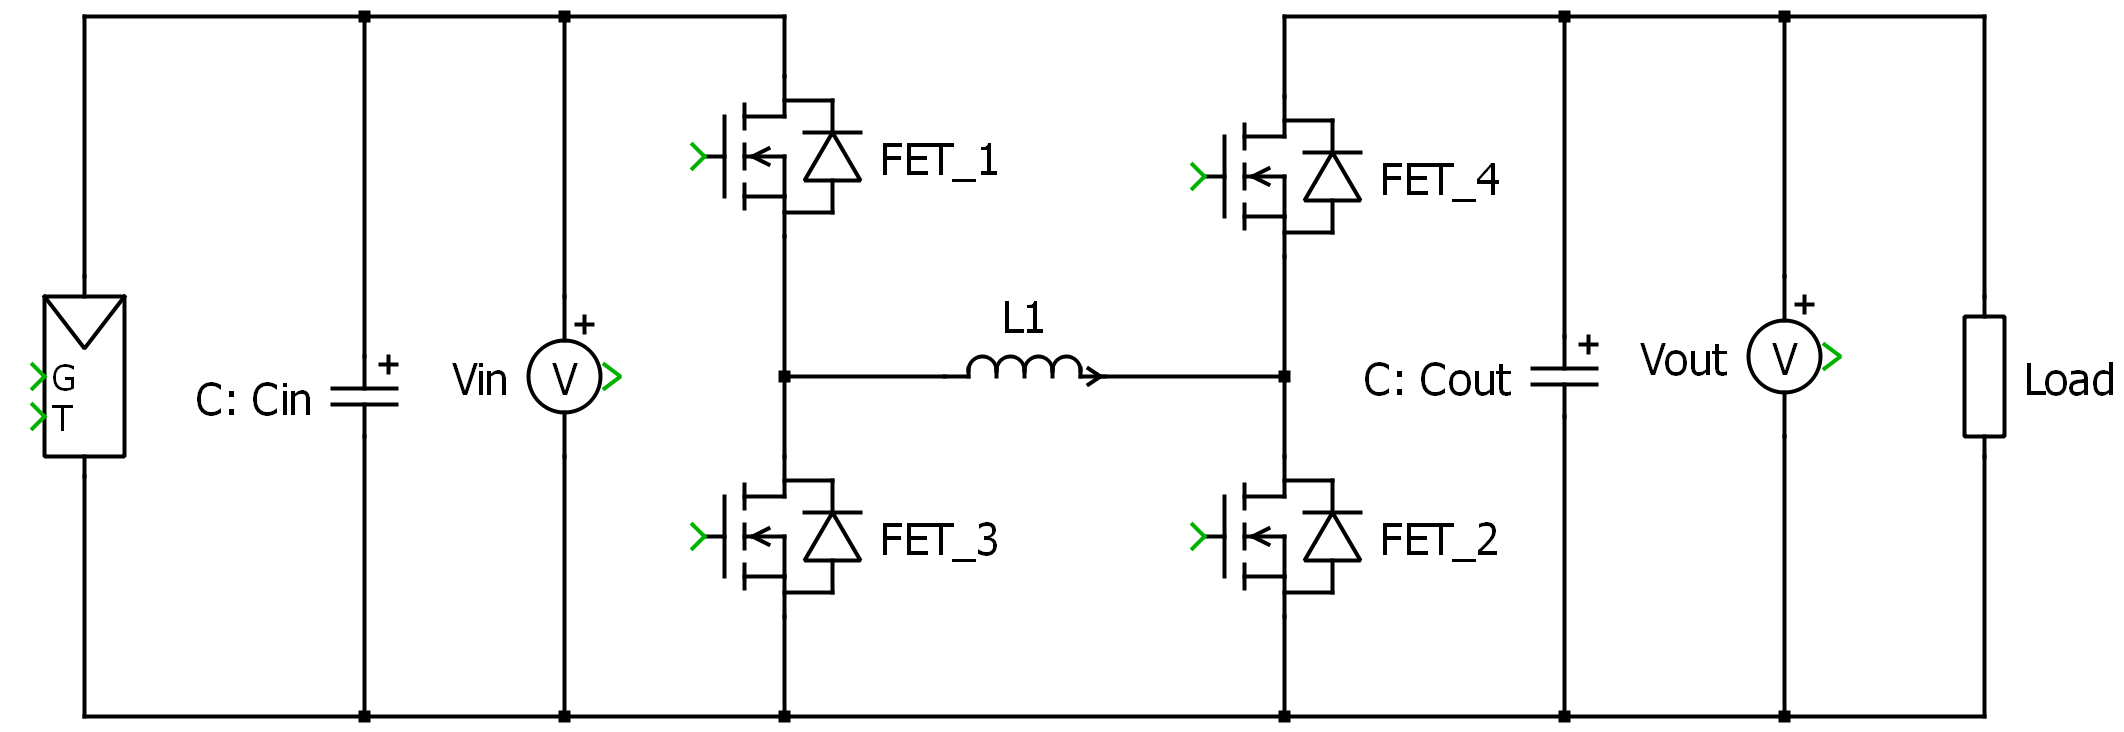
\includegraphics[width=0.7\linewidth]{../Pictures/P1/Sensors/voltage_sensors_placement.PNG}
		\caption{Voltage sensors placement}
		\label{fig:voltage_sensors_placement}
	\end{center}
\end{figure} 

\subsubsection{Voltage divider}
The input voltage at the voltage sensor is recommended to be in the range of $0V-2V$. To divide the measured voltage into that range, a voltage divider will be implemented. 

The maximum output voltage of the PV-module is the open-circuit voltage at $45.2V$. To achieve a safety margin and to make the converter adaptable to other types of PV-modules, $50V$ has been selected. The current flow in the voltage divider has been set at $1mA$, to secure a insignificant power loss. The resistors can be calculated with the following equations:
\begin{equation} \label{voltage_divider_R17_in}
	R_{17} = \frac{V_{in,max}-V_{out}}{I} = \frac{50V-2V}{1mA} = 48k\Omega
\end{equation}

\begin{equation} \label{voltage_divider_R18_in}
	V_{out} = V_{in,max} \cdot \frac{R_{18}}{R_{17}+R_{18}} \Rightarrow 2V = 50V \cdot \frac{R_{18}}{48k\Omega+R_{18}}
\end{equation}
\begin{center}
	$R_{18} = 1.958k\Omega$
\end{center}

To achieve these resistor values $R_{17} = 47k\Omega$ and $R_{18} = 2k\Omega$ have been chosen. 

\subsubsection{Filtering} \label{voltage_sensor_filter}
For a stable MPPT control, the measured voltage must have a very low ripple. To ensure this, a low-pass RC filter with a corner frequency at $500Hz$, will be placed between the voltage divider and the sensor. The resistor of the filter will be $R_{17}$ in the voltage divider. The capacitor will calculated as followed in equation \ref{voltage_sensor_in_filter_cap}:
\begin{equation} \label{voltage_sensor_in_filter_cap}
	C_{17} = \frac{1}{2\pi \cdot f_c \cdot R_{17}} = \frac{1}{2 \pi \cdot 500Hz \cdot 47k\Omega} = 6.7nF
\end{equation}

To achieve the capacitance $C_{17} = 6.6nF$ has been chosen. 

\subsubsection{Amplification} \label{voltage_sensor_amplification}
The input range of the ADC in the RT-Box is $0V-5V$. To take advantage of the full range an amplifier will be implemented. The output of the voltage sensor is differential with an offset at $1.23V$. Therefore a differential amplifier will be implemented using a LMC6484 quad operational amplifier. By using a quad amplifier, the same IC can be used for all the sensors. The relevant electrical specifications have been included in table \ref{tab:amplifier_specs}


\begin{table}[H]
	\centering
	\begin{tabular}{|p{6cm}|>{\centering}p{3.5cm}|>{\centering}p{3.5cm}|}
		\hline
		\rowcolor{lightgray}\multicolumn{3}{|l|}{ \textbf{Recommended ratings}} \\ \hline
		Supply voltage 	& $V_{DD}$ 		& $3-15.5$ [V]  \tabularnewline \hline
		Input voltage range & $V_{in}$ 	& $\pm V_{DD}$ [V]  \tabularnewline \hline
		
		\rowcolor{lightgray}\multicolumn{3}{|l|}{ \textbf{Other values of interest}} \\ \hline
		Slew rate 					& $SR$ 	& $1.3$ [$V/\mu s$]  \tabularnewline \hline
		Gain-Bandwith product 		& $GBW$ & $1.5$ [$MHz$]		\tabularnewline \hline
		Number of amplifiers 		&  	--	& $4$ [-]			\tabularnewline \hline
		Package 					&  	--	& SOIC [-] 				\tabularnewline \hline
		
	\end{tabular}
	\caption{Electrical specifications LMC6484 \cite{sensor_opamp}}
	\label{tab:amplifier_specs}
\end{table}

The resistors of the differential amplifier will be sized with equation \ref{voltage_sensor_gain}.
\begin{equation} \label{voltage_sensor_gain}
	V_{out} = \frac{R_{22}}{R_{20}} \cdot (V_2-V_1)
\end{equation}

Where $V_2-V_1$ is the difference between the output pins of the voltage sensor. With unity gain in the voltage sensor, the maximum difference at the output will be $2V$. This should correspond to the maximum input voltage of the ADC at $5V$. $R_1$ is selected to be $11k\Omega$. The resistor $R_{22}$ is now calculated using equation \ref{voltage_sensor_gain}.
\begin{equation}
	5V = \frac{R_{22}}{11k\Omega} \cdot 2V
\end{equation}
\begin{center}
	$R_{22} = 27.5k\Omega$
\end{center}
To achieve the value of $R_{22}$ it's rounded to be $27k\Omega$. Furthermore $R_{19} = R_{20}$ and $R_{21} = R_{22}$, to get a balanced differential amplifier.

\subsubsection{The circuit}
The circuit regarding the input voltage measurement is shown at figure \ref{fig:input_voltage_sensor_circuit}. $V_{in}$ is the measured voltage from the PV-module. The points $OA1_+$ and $OA1_-$ are connected to the non-inverting and inverting input of the amplifier respectively. $OA1_{out}$ is connected to the output of the amplifier. $C_{15}$ and $C_{16}$ are decoupling capacitors for the two supply voltages. The maximum input voltage of the voltage sensor is $5V$. Because of this a $4.7V$ zener diode has been added at the input, to protect it from over-voltage.

\begin{figure}[H]
	\begin{center}
		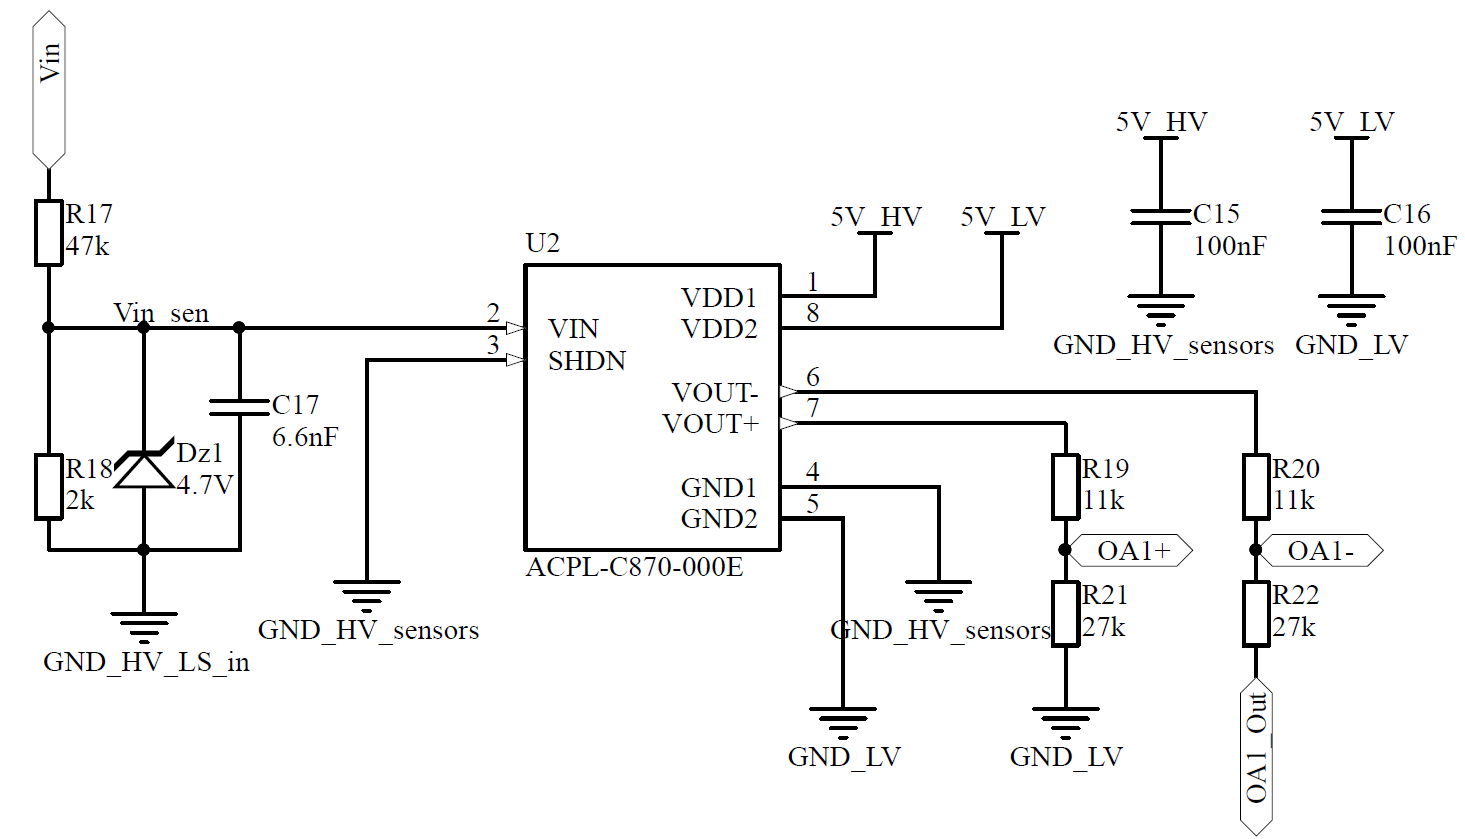
\includegraphics[width=0.7\linewidth]{../Pictures/P1/Sensors/input_voltage_sensor.PNG}
		\caption{Input voltage sensor}
		\label{fig:input_voltage_sensor_circuit}
	\end{center}
\end{figure}

\subsection{Output voltage sensor}
The voltage sensor at the output is design by the same procedure as the input sensor. The voltage divider will designed such that the values of the amplifier can be reused.

\subsubsection{Voltage divider}
The maximum output voltage of the DC/DC converter will be $90V$, when only 4 PV-modules are used. To insert a safety margin if one converter fails, the maximum sensed voltage will be designed at $120V$.

The resistors will be sized by reusing equation \ref{voltage_divider_R17_in} and \ref{voltage_divider_R18_in}.
\begin{equation}
	R_{26} = \frac{V_{in,max}-V_{out}}{I} = \frac{120V-2V}{1mA} = 118k\Omega	
\end{equation}

\begin{equation} 
	V_{out} = V_{in,max} \cdot \frac{R_{27}}{R_{26}+R_{27}} \Rightarrow 2V = 120V \cdot \frac{R_{27}}{118k\Omega+R_{27}}
\end{equation}
\begin{center}
	$R_{27} = 2.03k\Omega$
\end{center}

To achieve these resistor values $R_{26} = 120k\Omega$ and $R_{27} = 2k\Omega$ have been chosen. 

\subsubsection{Filtering}
The filter will be design with the same corner frequency at $500Hz$, as for the input sensor.

The resistor of the filter will be $R_{26}$ in the voltage divider. The capacitor will be calculated as followed in equation \ref{voltage_sensor_out_filter_cap}:
\begin{equation} \label{voltage_sensor_out_filter_cap}
	C_{22} = \frac{1}{2\pi \cdot f_c \cdot R_{26}} = \frac{1}{2 \pi \cdot 500Hz \cdot 120k\Omega} = 2.6nF
\end{equation}

To achieve the capacitance $C_{22} = 3.3nF$ has been chosen. 

\subsubsection{The circuit}
The circuit regarding the input voltage measurement is shown at figure \ref{fig:output_voltage_sensor_circuit}. 

\begin{figure}[H]
	\begin{center}
		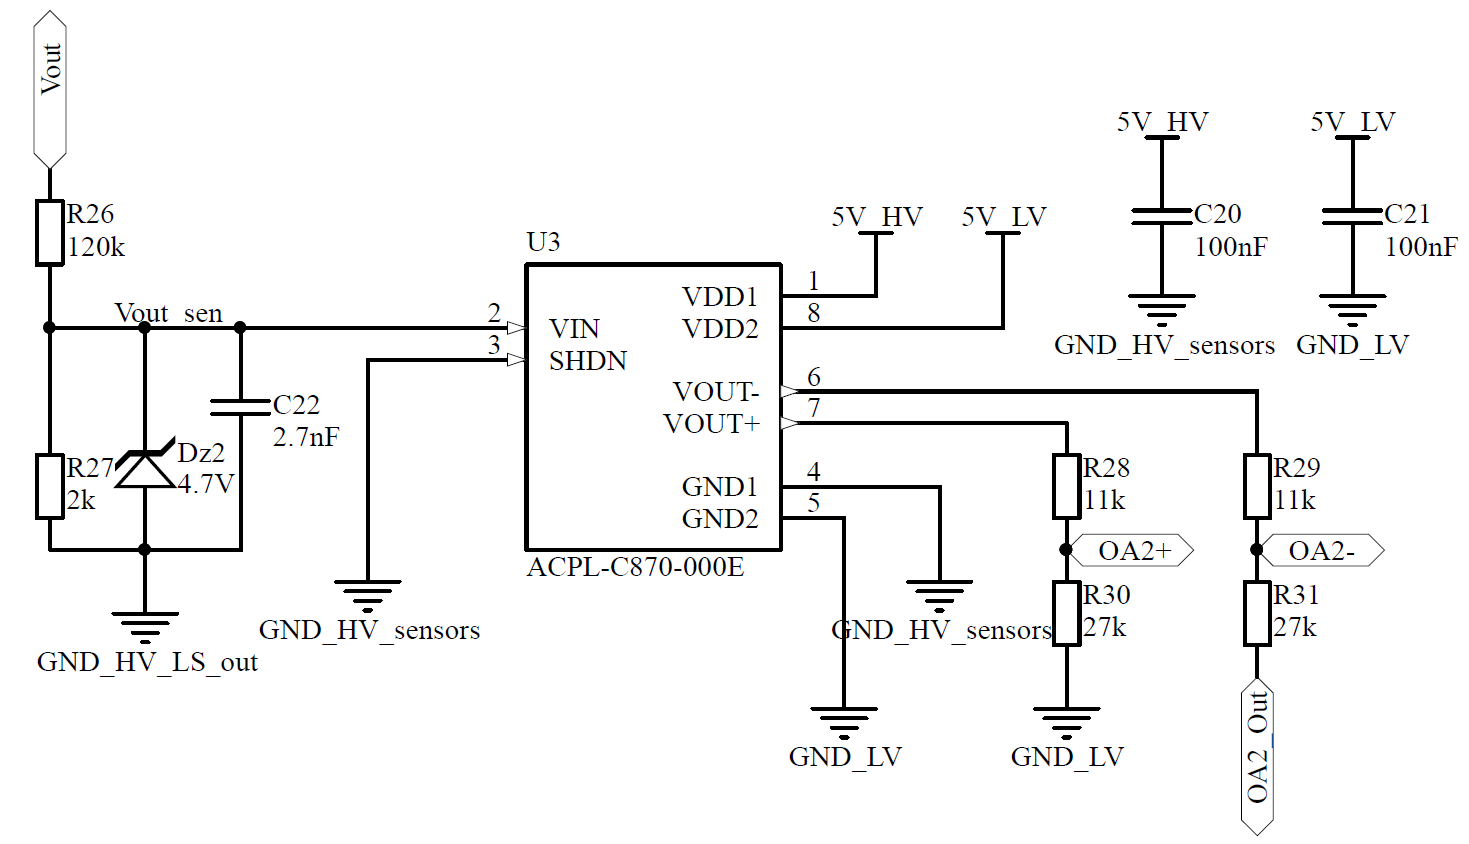
\includegraphics[width=0.7\linewidth]{../Pictures/P1/Sensors/output_voltage_sensor.PNG}
		\caption{Output voltage sensor}
		\label{fig:output_voltage_sensor_circuit}
	\end{center}
\end{figure}